\section{Preprocessing}

\subsection*{Q1: Preprocessing (2 pt)}
\textit{After familiarizing yourself with the TweetsCOV19 dataset, explain your data pre-processing steps for the following parts of the project. Provide code snippets for each pre-processing step. Comment on possible challenges posed by using the raw Twitter data, such as irregular capitalization, variable declination of words, spelling mistakes, punctuation, urls, mentions, emojis, abbreviations and others. Describe whether these apply to this corpus, and how you handled them if so.}

As a first step in our preprocessing pipeline, we enforced the data types of each column and dropped rows (or tweets) that did not follow such a table schema, or were duplicates. We found that about 126K tweets were duplicates, while about 53K tweets had invalid TweetIDs or invalid indices. Finally, we dropped about 113K tweets that contained the value 'NaN' in any of the columns, as a 'NaN' in a column can be indicative of data corruption for that tweet (as we had a very large dataset, we deemed it appropriate to have this stringent procedure). We thus end up with approximately 382K tweets out of an original 675K.

The dataset has quite a lot of challenges, even after dropping invalid rows as above: indeed, the TweetText column is very unstructured by nature, as it can contain URLs, emojis, user mentions, hashtags, misspellings, abbreviations, numbers, and variations in capitalisation. In order to counter this, we used a combination of regex and string functions to very efficiently strip the tweets of URLs, mentions, numbers, capitalisation, emojis, and to split hashtags into separate words, done in a few seconds. An example of this procedure is shown in Figure \ref{fig:prepr}, and the code snippet to achieve this is shown as well \cref{listing:p1-code1}.


\begin{listing*}[t]
\begin{minted}{python}
def rep(m):
   s=m.group(1)
   return ' '.join(re.split(r'(?=[A-Z])', s))


df_tweets['TweetText'] = [re.sub('((www\.[^\s]+)|(https?://[^\s]+))', '', x) for x in df_tweets['TweetText']] #remove url
df_tweets['TweetText'] = [re.sub('@[^\s]+', '' , x) for x in df_tweets['TweetText']] #remove mentions
df_tweets['TweetText'] = [x.encode("ascii", "ignore").decode() for x in df_tweets['TweetText']] # remove emojis
df_tweets['TweetText'] = [re.sub(r'#(\w+)', rep, x) for x in df_tweets['TweetText']] # split hashtags that are stuck together if they have case change: #iLovePotatoes becomes i love potatoes
df_tweets['TweetText'] = [re.sub(r'\W+', ' ', x) for x in df_tweets['TweetText']] # remove all characters that aren't alphanumerical - hashtag signs, punctuation, slashes...
df_tweets['TweetText'] = df_tweets["TweetText"].astype(str).str.replace('\d+', '') # remove numbers entirely
df_tweets['TweetText'] = df_tweets['TweetText'].str.lower() # remove all caps
\end{minted}
\caption{}
\label{listing:p1-code1}
\end{listing*}

\begin{figure}
    \centering
    \begin{subfigure}{0.5\columnwidth}
        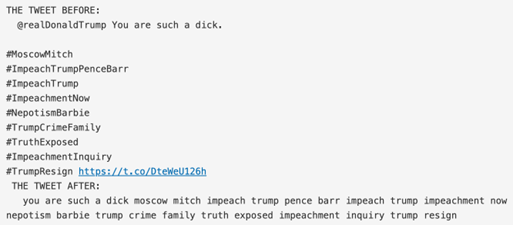
\includegraphics[width=1\textwidth]{images/prepr1.png}
    \end{subfigure}
    \caption{}
    \label{fig:prepr}
\end{figure}


We then tokenize each of the tweets by using Nltk's tokenize package, and then remove common English stopwords using Nltk's corpus package.
The column 'UserLocation' is used in Part 3, where we filtered tweets based on location, which we don't consider to be a part of preprocessing, however this is fully explained in Part 3. 

Finally, we choose to split our labels into two different columns, one for positive and for negative, as this is the obvious choice in order to use supervised models with two output heads, instead of being boxed into carrying out classification over 25 possible output labels (5*5).


\subsection*{Q2: Exploratory data analysis (1 pts)}
\textit{Perform a short data analysis of the TweetsCOV19 dataset. In particular, what are the most common uni- and bi-grams in the corpus before and after preprocessing? How does this word distribution vary as a function of the sentiment labels? What is the proportion of each sentiment? Think about how best to visualize this and summarize your findings.}

The most common unigrams and bigrams after preprocessing are shown in Figure \ref{fig:uni_bi_af}, and the ones before preprocessing are shown in Figure \ref{fig:uni_bi_bef} (after removing invalid rows as explained above). We show the two words in a bigram separated by an underscore, for better visualization in the word cloud. As expected, the observed unigrams and bigrams are worthless before preprocessing.

\begin{figure}
    \centering
    \begin{subfigure}{0.49\columnwidth}
        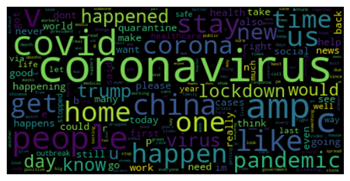
\includegraphics[width=1\textwidth]{images/uni_af.png}
    \end{subfigure}
    \centering
    \begin{subfigure}{0.49\columnwidth}
        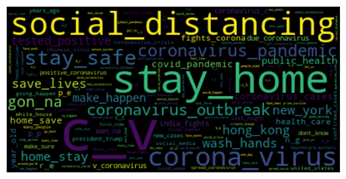
\includegraphics[width=1\textwidth]{images/bi_af.png}
    \end{subfigure}
    \caption{Most common unigrams (left) and most common bigrams (right) \textbf{after tweet preprocessing} shown as word clouds.}
    \label{fig:uni_bi_af}
\end{figure}

\begin{figure}
    \centering
    \begin{subfigure}{0.49\columnwidth}
        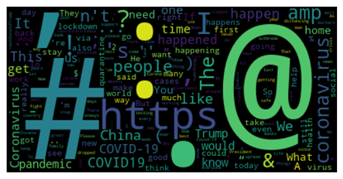
\includegraphics[width=1\textwidth]{images/uni_bef.png}
    \end{subfigure}
    \centering
    \begin{subfigure}{0.49\columnwidth}
        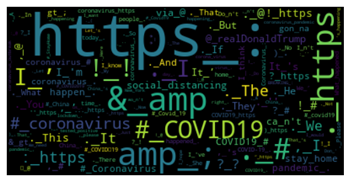
\includegraphics[width=1\textwidth]{images/bi_bef.png}
    \end{subfigure}
    \caption{Most common unigrams (left) and most common bigrams (right) \textbf{before tweet preprocessing} shown as word clouds.}
    \label{fig:uni_bi_bef}
\end{figure}

We then follow exactly the same procedure, but for extremely negative tweets, shown in Figure \ref{fig:uni_bi_neg}, and for extremely positive tweets, shown in Figure \ref{fig:uni_bi_pos}.

\begin{figure}
    \centering
    \begin{subfigure}{0.49\columnwidth}
        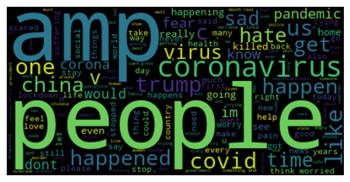
\includegraphics[width=1\textwidth]{images/uni_neg.png}
    \end{subfigure}
    \centering
    \begin{subfigure}{0.49\columnwidth}
        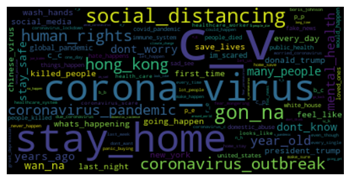
\includegraphics[width=1\textwidth]{images/bi_neg.png}
    \end{subfigure}
    \caption{Most common unigrams (left) and most common bigrams (right) for \textbf{extremely negative tweets} (negative\_sentiment $<$ -3).}
    \label{fig:uni_bi_neg}
\end{figure}

\begin{figure}
    \centering
    \begin{subfigure}{0.49\columnwidth}
        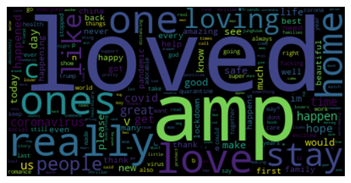
\includegraphics[width=1\textwidth]{images/uni_pos.png}
    \end{subfigure}
    \centering
    \begin{subfigure}{0.49\columnwidth}
        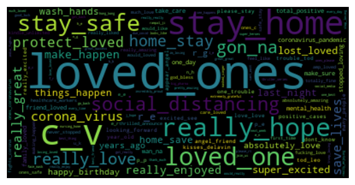
\includegraphics[width=1\textwidth]{images/bi_pos.png}
    \end{subfigure}
    \caption{Most common unigrams (left) and most common bigrams (right) for \textbf{extremely positive tweets} (positive\_sentiment $>$ 3).}
    \label{fig:uni_bi_pos}
\end{figure}

One can observe the unigram 'amp' in every unigram word cloud, however this is a keyword in social media websites (Accelerated Mobile Pages) and is thus not significant. We observe that the negative tweets have many terms with negative connotations on social media ('hate', 'sad', 'killed', 'Trump') but also neutral words like 'people', 'coronavirus', 'covid', which are words that do not appear in the extremely positive unigram word cloud. This shows that \textbf{tweets that mention the COVID-19 pandemic explicitly tend to be more overtly negative}. The extremely positive tweets' word clouds show very positive terms like 'loved', 'loving', 'stay home', 'stay safe', 'one', 'protect loved', and thus refer more to enforcing a positive attitude during the pandemic rather than the events of the pandemic themselves. 

We show the proportion of each sentiment label as a bubble chart along a grid defined by the labels (we take the absolute value of the negative sentiments, plotted here on the y-axis), in Figure \ref{fig:bubble}. We observe that \textbf{most of the labels are fairly neutral} (leaning towards the low end of the positive and negative values), however, the \textbf{more extreme tweets tend to be more negative than positive}: for example, (1, 4) is larger than (4, 1), where (x, y) refers to the bubble size of positive\_sentiment = x and negative\_sentiment = y. The dataset thus contains a very large proportion of mild tweets that are not particularly charged in sentiment.

\begin{figure}
    \centering
    \begin{subfigure}{0.7\columnwidth}
        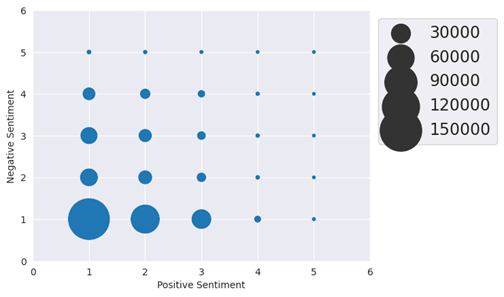
\includegraphics[width=1\textwidth]{images/bubble.png}
    \end{subfigure}
    \caption{Bubble chart of the number of positive and negative sentiments in the dataset.}
    \label{fig:bubble}
\end{figure}

\subsection*{Q3: Metric choice (1 pt)}
\textit{Are the classes balanced? Choose and justify your evaluation metric(s) for the analysis of sentiment performed in the following parts of the project. Provide a code snippet used to produce performance measurements using the chosen metric.}

First, we introduce our interpretation of the problem. Predicting a value for either positive or negative sentiment is inherently a regression problem since the integer value is ordinal rather than categorical. In other words, the \textit{positive sentiment} value of $3$ semantically lies between the values of $2$ and $4$. The fact that these five categories of values (for both sentiments) are ordered brings the potential for models to perform better. However, in the problem description, we are given the task to solve a classification problem. Hence, we decided for the following approach:
\begin{enumerate}
    \item We are \textbf{solving a classification problem} as is asked for, in that our models return two integers in the suitable ranges (one for positive and negative sentiment), and during evaluation, we will treat each sentiment variable as categorical, therefore only allowing categorical metrics.
    \item Under the hood, we allow the models to capture the intrinsic regression problem, even though their output for evaluation will be one of five classes. This means that if it is suitable for a given model, we will naturally choose a regression loss function such as the mean squared error.
\end{enumerate}

\textbf{Metric choice.}
At first, we observe from \cref{fig:bubble} that classes are highly imbalanced, with classes closer to zero being orders of magnitude more likely (for both sentiment variables). Therefore an appropriate metric has to take the class imbalance into account. For a given class, a natural choice is first to evaluate the standard F1 score, calculated from Precision and Recall, and then calculate the Weighted F1 score which takes class imbalance into account. However, considering all 25 classes individually (= all combinations of permissible values for positive and negative sentiment variables) would not lead to a representative metric because a model that predicts both variables incorrectly would be rated the same as another model which predicts one of the variables correctly. Therefore, we decided to split the problem into two separate classification problems, one for each sentiment variable. We then calculate the Weighted F1 score for both variables and report their harmonic mean as the final metric. The harmonic mean, as opposed to the arithmetic mean, penalises models whose performance on the two variables is imbalanced.

\begin{listing*}[t]
\begin{minted}{python}
from sklearn.metrics import f1_score
from scipy.stats import hmean

def f1w_hm(pos_true, pos_pred, neg_true, neg_pred):
    """Harmonic mean of the weighted f1 scores for positive and negative sentiment variables.

    Args:
        pos_true (np.array): True labels of the positive sentiment variable.
        pos_pred (np.array): Predicted labels of the positive sentiment variable.
        neg_true (np.array): True labels of the negative sentiment variable.
        neg_pred (np.array): Predicted labels of the negative sentiment variable.
    """
    pos_f1 = f1_score(pos_true, pos_pred, average='weighted')
    neg_f1 = f1_score(neg_true, neg_pred, average='weighted')
    return hmean([pos_f1, neg_f1])
\end{minted}
\caption{The "Weighted-F1 HM" metric chosen for the two-output classification problem of predicting the positive and negative sentiment variables.}
\label{listing:p1-metric}
\end{listing*}

\Cref{listing:p1-metric} shows the primary metric that we call \textit{Weighted-F1 HM} that we will use to evaluate a model's performance on the given classification task, as well as to compare the predictive performance of different models.


\subsection*{Q4: Dataset splitting (1 pt)}
\textit{Split your dataset into a training, validation and test set. Motivate your approach for this, comment on possible evaluation challenges (e.g. label shift over time).}

We choose to split our dataset in the following manner: we reserve 33\% of the dataset for the test set, and keep 67\% of the dataset for training and validation (where validation is typically 20\% of the training set, however this has been varied in our experiments). We also split by randomly shuffling the dataset, as we want the training to be agnostic to the timeframe. Indeed, in Figure \ref{fig:av_pos}, we plot the average of the positive labels in time (sorted timestamps, then averaged over 200 bins), and observe that this average isn't constant: there is a sharp fall towards the middle of the dataset. Thus, if we split our dataset without shuffling, we risk ending up with dataset splits that have different label proportions with respect to each other.

\begin{figure}
    \centering
    \begin{subfigure}{0.5\columnwidth}
        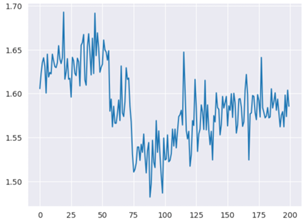
\includegraphics[width=1\textwidth]{images/av_pos.png}
    \end{subfigure}
    \caption{Average of positive labels over time, over 200 bins.}
    \label{fig:av_pos}
\end{figure}